\begin{frame}
    \frametitle{Convergence}
    \begin{center}
	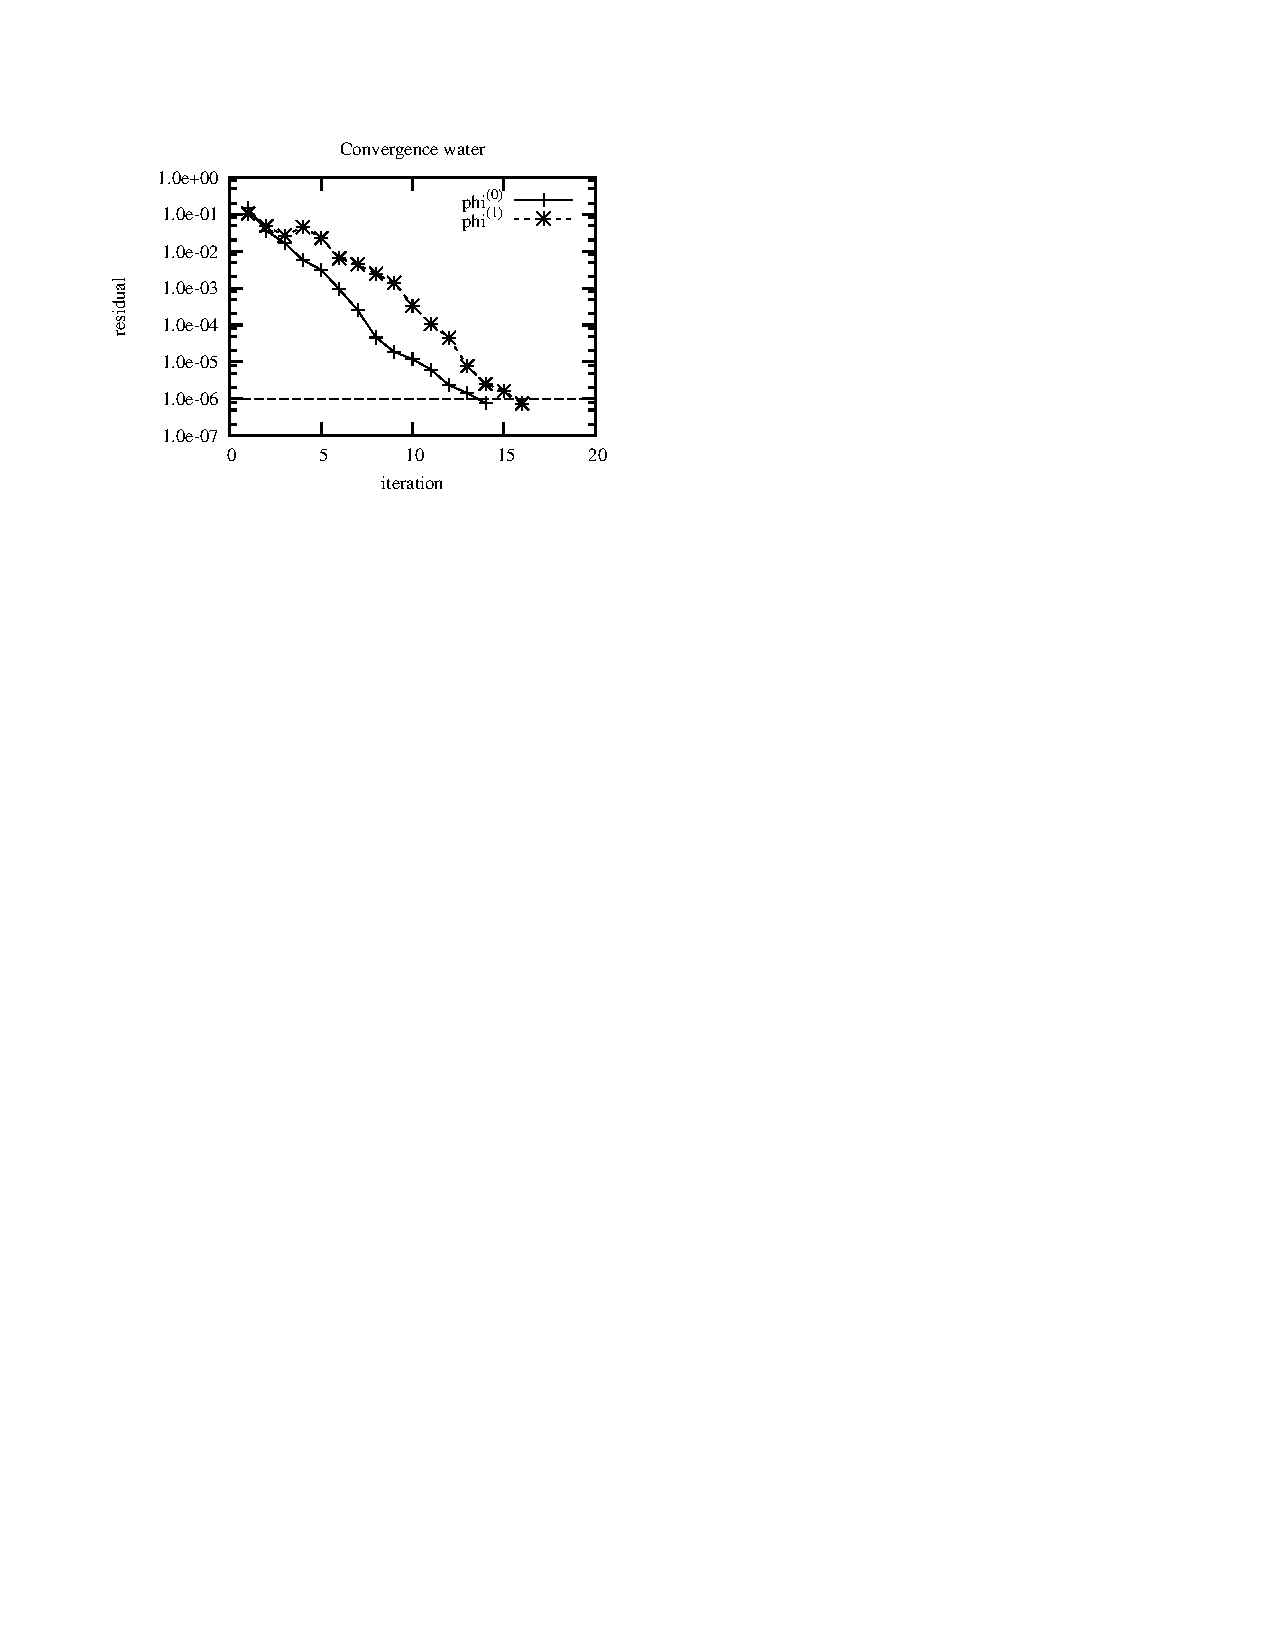
\includegraphics[scale=1.0, clip, viewport = 50 550 300 730]{figures/response_convergence.pdf}
    \end{center}
\end{frame}

\begin{frame}
    \frametitle{Accuracy and origin dependence}
    \centering
    \textbf{Hartree-Fock magnetizability (a.u.) of water}
    \begin{table}
    \scriptsize
    \begin{tabular}{cccrrr}
    \hline
    \hline                                  
        &               &                   &                 &                  &                  \\
        &               &                   &
    \multicolumn{3}{c}{$r_O=(0, 0, 0)$ }    \\
    \cline{4-6}                             
    $k$ &$\epsilon$ &$\Delta\phi$           &
    \multicolumn{1}{c}{$\xi^{dia}$}	    &
    \multicolumn{1}{c}{$\xi^{para}$}        &
    \multicolumn{1}{c}{$\xi^{tot}$}	    \\
        &               &                   & \hspace{15mm}   & \hspace{15mm}    & \hspace{15mm}    \\
    \hline
        &               &                   &                 &                  &                  \\
    5 & $10^{-3}$       & $10^{-2}$         & -3.269 \red{608}& 0.32\red{5 099}  & -2.94\red{4 509} \\
    7 & $10^{-5}$       & $10^{-4}$         & -3.269 110      & 0.322 3\red{56}  & -2.946 7\red{54} \\
    9 & $10^{-7}$       & $10^{-6}$         & -3.269 110      & 0.322 364        & -2.946 746       \\
        &               &                   &                 &                  &                  \\
    \multicolumn{2}{l}{aug-cc-pV6Z}& (443)  & -3.2691         & 0.3224           & -2.946\red{8}    \\
    \multicolumn{2}{l}{aug-cc-pVQZ}& (172)  & -3.27\red{01}   & 0.322\red{3}     & -2.94\red{79}    \\
    \multicolumn{2}{l}{aug-cc-pVDZ}&  (41)  & -3.2\red{824}   & 0.32\red{51}     & -2.9\red{573}    \\
        &               &                   &                 &                  &                  \\
    \hline
    \hline
    \end{tabular}
    \end{table}
    GTO (GIAOs) calculations with Dalton
\end{frame}

\begin{frame}
    \frametitle{Accuracy and origin dependence}
    \centering
    \textbf{Hartree-Fock magnetizability (a.u.) of water}
    \begin{table}
    \scriptsize
    \begin{tabular}{cccrrr}
    \hline
    \hline                                  
        &               &                   &                    &                  &                  \\
        &               &                   &
    \multicolumn{3}{c}{$r_O=(5, 5, 5)$ }    \\
    \cline{4-6}                             
    $k$ &$\epsilon$ &$\Delta\phi$           &
    \multicolumn{1}{c}{$\xi^{dia}$}	    &
    \multicolumn{1}{c}{$\xi^{para}$}        &
    \multicolumn{1}{c}{$\xi^{tot}$}	    \\
        &               &                   & \hspace{15mm}      & \hspace{15mm}    & \hspace{15mm}    \\
    \hline
        &               &                   &                    &                  &                  \\
    5 & $10^{-3}$       & $10^{-2}$         & -127.84\red{0 649} & 124.90\red{6 519}& -2.9\red{34 131} \\
    7 & $10^{-5}$       & $10^{-4}$         & -127.846 5\red{82} & 124.900 \red{435}& -2.946 \red{147} \\
    9 & $10^{-7}$       & $10^{-6}$         & -127.846 564       & 124.899 8\red{54}& -2.946 7\red{10} \\
        &               &                   &                    &                  &                  \\
    \multicolumn{2}{l}{aug-cc-pV6Z}& (443)  & -127.846\red{6}    & 123.\red{7548}   & \red{-4.0918}    \\
    \multicolumn{2}{l}{aug-cc-pVQZ}& (172)  & -127.84\red{76}    & 12\red{0.5026}   & \red{-7.3450}    \\
    \multicolumn{2}{l}{aug-cc-pVDZ}&  (41)  & -127.8\red{713}    &  \red{98.7552}   & \red{-29.1161}   \\
        &               &                   &                    &                  &                  \\
    \hline
    \hline
    \end{tabular}
    \end{table}
    GTO (no GIAOs) calculations with Dalton
\end{frame}

\begin{frame}
\frametitle{A difficult case}
   
\centering
\textbf{Hartree-Fock shielding constant (ppm) of magnesium oxide}
\begin{table}
\scriptsize
\begin{tabular}{cccrr}
\hline
\hline
    &           &                     &               &               \\
$k$ &$\epsilon$ &$\Delta\phi$   &
\multicolumn{1}{c}{$\sigma(Mg)$}&
\multicolumn{1}{c}{$\sigma(O)$}	\\
    &           &                     &               &               \\
\hline                                
    &           &                     &               &               \\
  6 & $10^{-4}$ & $10^{-3}$           &  15\red{38.9211}   & -1\red{6726.3490}   \\
  7 & $10^{-5}$ & $10^{-4}$           &  158\red{4.1109}   & -17\red{466.4867}   \\
  8 & $10^{-6}$ & $10^{-5}$           &  1578.\red{7322}   & -173\red{58.6849}   \\
  9 & $10^{-7}$ & $10^{-6}$           &  1579.4\red{610}   & -1737\red{5.4221}   \\
    &           &                     &               &               \\
\multicolumn{2}{r}{aug-pcS-4} &(260)  &  16\red{05.7661}   & -17\red{904.0731}   \\
\multicolumn{2}{r}{aug-pcS-3} &(162)  &  1\red{719.9701}   & -2\red{0055.5992}   \\
\multicolumn{2}{r}{aug-pcS-2} & (86)  & \red{ 4282.4997}   & \red{-69183.9283}   \\
\multicolumn{2}{r}{aug-pcS-1} & (46)  & \red{-1173.7349}   & \red{ 10814.1557}   \\
\multicolumn{2}{r}{aug-pcS-0} & (27)  & \red{  254.9829}   & \red{ 36289.8265}   \\
    &           &                     &               &               \\
\hline
\hline
\end{tabular}
\end{table}

Frank Jensen's polarization consistent basis sets\\
GTO calculations with Dalton

\end{frame}
